% fig1_system_rev.tex - Fig. 1 of the letter (standalone TikZ), one-column layout, 2026-11-17.
% Build: latexmk -pdf -outdir=out fig1_system_rev.tex ; cp out/fig1_system_rev.pdf fig_cl/
% Layout: one column, printed at width=\columnwidth (scale 1.0): the canvas is pinned to the IEEEtran
% column, 252 pt = 88.57 mm, so every size below is the printed size. Transmitter chain of user u (top
% row: BERT and centering (1) in one block, PCA V^T, placement i_u(t), and the mask block, which computes
% omega_u[tau] by (P) and carries the energy E_u), the channel column (gain g_{u,s}, adder with the noise
% n and the other users), the receiver row: joint LMMSE with the side inputs Psi[tau] (gains times mask
% values of all users) and Gamma, inverse V, and the mask design (P), whose dashed announcement (U,
% gamma, g_{u,s}, scene) lets every transmitter compute its placement and mask of the frame by the same
% closed form; below it, spanning the full column width, the time-frequency map of the real-valued masks
% of ALL active users over the N = 24 slots (columns) of four consecutive frames tau, tau+1, tau+2, tau+3
% (rows: aged gains, overload, fresh gains, one scene).
% Mask map: color = user (1 blue, 2 orange, 3 green, 4 coral red, 5 dark violet, 6 light cyan;
% gray levels 0.299R+0.587G+0.114B about 0.43, 0.64, 0.24, 0.53, 0.11, 0.80, so neighbouring
% users of the overload row differ by at least 0.21 and any two users by at least 0.10), white =
% silent use. Every used cell holds a bar whose height is the RMS amplitude omega*sqrt(lambda_i)
% that the mask gives the uses of that slot, on one scale for all rows (a mask value omega grows
% as lambda_i^{-1/2} for weak coefficients, so the amplitude shows the share of a use; within one
% use the ratio of two users' amplitudes equals the ratio of their mask values).
% The heights follow from the allocation (16) on the load masks (5) (label eq:wf; Code/fig1_amplitudes.py calls it (12)),
% the channel-aware masks (19) (label eq:wfcsi) and the overlapping masks (18) (label eq:Wi) of the
% manuscript, evaluated on the held-out test spectrum (the training-pool eigenvalues change no bar
% amplitude by more than 0.072, at the smallest tau bar: 0.14 mm at \ys = 2.0 mm, 0.08 mm at the
% earlier print scale; see Code/fig1_amplitudes.py), bar height = \ys times the RMS amplitude:
%   frame tau,   U = 2, aged gains, 10 dB: load masks, slot s used by the user of rank s mod 2 and
%                carrying group floor(s/2) mod 6, values from (16) with two copies per
%                coefficient (held-out AG News spectrum data/effdim_spectrum_test.npy, energy
%                d_s/U = 1536); \ampT is reproduced by Code/fig1_amplitudes.py;
%   frame tau+1, U = 6 > K = 4 (overload), 10 dB: load masks, slot s used by the user of rank
%                s mod 6 (users 1-6 = ranks 0-5) and carrying group floor(s/6), so rank j sends
%                the groups 0, 1, 2, 3 of its code on the slots j, j+6, j+12, j+18 (d_u = 512
%                coefficients, one copy each, energy d_s/U = 512) and its groups 4 and 5 are cut;
%                the gains of the four joining users are not yet reported (aged or unsounded), so
%                (P) returns the load masks here; with fresh gains it would pick channel-aware
%                masks at U = 6 (coherence paragraph of Section IV-B);
%                bar = sqrt(mean of P_i over the 128 coefficients of the group) from (16) on the
%                same spectrum, \ampO = 1.519, 0.935, 0.708, 0.564 (Code/fig1_amplitudes.py);
%   frame tau+2, U = 3, fresh gains, 10 dB, beta_u = 1: channel-aware masks; greedy support
%                growth on the gains |h_{u,s}| below (8 slots per user), each user sends its six
%                groups once on its six strongest slots with the values (19), and its two extra
%                slots stay silent; one gain strip per user above the row (user 1, 2, 3 from top,
%                one neutral ramp, darker = stronger), the darkest strip of every used slot
%                belongs to the user of that slot;
%   frame tau+3, U = 2, one scene, 0 dB: the overlapping masks (18) for an illustrative strongly
%                shared scene, kappa_i = 0.8 for every coefficient (mixture setting --mix 0.8,
%                observers with strongly shared content such as cameras of one scene), so the
%                common mode has a_0 = 1 + kappa = 1.8 and the difference mode a_1 = 1 - kappa =
%                0.2; COCO group energies (data/shared/content_stats.json, uniform within a group),
%                total energy 3072 over both users, on the common repetition placement; the
%                realization W_i is split over the pairs of copies (0,1) and (2,3), so the dominant
%                user alternates over the copies and a use carries (sqrt(p_0) +- sqrt(p_1))/(2 sqrt 2);
%                group 0 has one dominant and one smaller same-sign value per use (overlap index
%                t = (p_0 - p_1)/(p_0 + p_1) = 0.25), groups 1-5 have zero difference-mode energy
%                and two equal values (t = 1, full superposition), so every slot carries both users.
% Scale and sizes: block text and arrow labels 8 pt (math
% scripts 7.05 pt), every other text 7.05 pt, so no glyph prints below 7 pt (7.02 bp in the PDF).
% Edge labels b_u, c_u, r_u (transmitter) and y, c_hat_u (receiver) sit at pos 0.42 of their arrows
% (toward the source, away from the arrowhead) and Psi[tau], Gamma at the middle of its arrow, 3.8 pt
% left of the shaft (it keeps 1.9 pt from the mask design block above), so every label ink keeps at
% least 3.1 pt from its arrowhead (transmitter arrows 7.6 mm long); the dotted 'other users' arrow has
% a visible shaft. Slot width 2.86 mm (was 1.5 mm at scale 0.8655 = 1.30 mm printed). Bar heights: the same RMS
% amplitudes \ampT, \ampO, \slotamp, \ampD, \ampS as before, times one uniform scale \ys = 2.0 mm (was
% 1.25 mm), cell heights scaled by the same factor 1.6 (2.8 -> 4.48 mm, 3.1 -> 4.96 mm), gain strips
% 0.55 -> 0.88 mm.
\RequirePackage{fix-cm}% scalable Computer Modern, so the math sizes below exist
\documentclass[tikz,border=0pt]{standalone}
\usepackage{amsmath,amssymb,bm}
% no glyph below 7 bp (PDF points; 7.05 TeX pt = 7.02 bp): scripts of the 8 pt blocks and labels and of
% the 7.05 pt labels at 7.05 pt
\DeclareMathSizes{8}{8}{7.05}{7.05}
\DeclareMathSizes{7.05}{7.05}{7.05}{7.05}
\usetikzlibrary{arrows.meta,positioning,calc,fit,backgrounds}
% user colors, distinct in hue and in gray level
\definecolor{uA}{rgb}{0.25,0.42,0.92}% user 1, blue
\definecolor{uB}{rgb}{0.96,0.58,0.12}% user 2, orange
\definecolor{uC}{rgb}{0.05,0.36,0.14}% user 3, green
\definecolor{uD}{rgb}{0.95,0.35,0.40}% user 4, coral red
\definecolor{uE}{rgb}{0.24,0.00,0.36}% user 5, dark violet
\definecolor{uF}{rgb}{0.58,0.89,0.96}% user 6, light cyan
\newcommand{\sw}[1]{\textcolor{#1}{\rule{1.9mm}{1.9mm}}}% color swatch of the key
\begin{document}
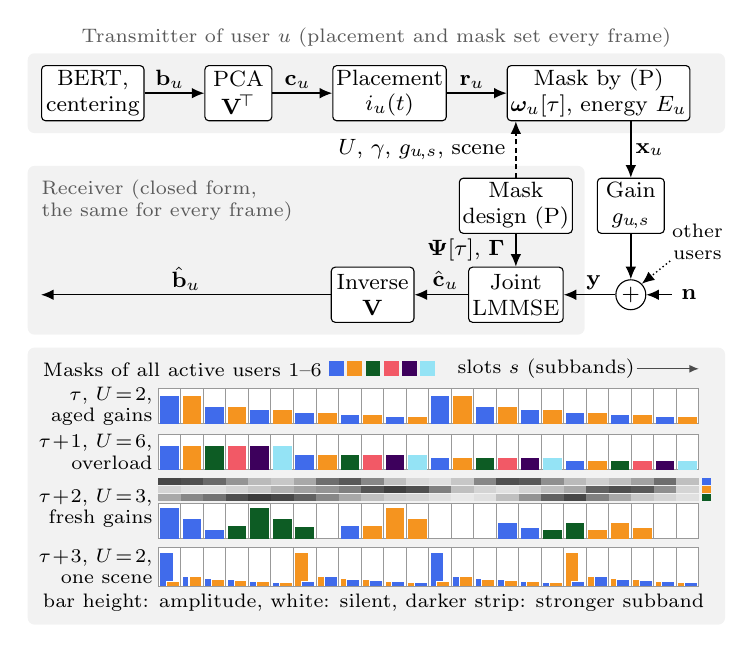
\begin{tikzpicture}[x=1mm,y=1mm,
  font=\fontsize{8}{9.2}\selectfont,
  blk/.style={draw,rounded corners=1.4pt,minimum height=7.0mm,inner sep=1.2pt,align=center,fill=white},
  sum/.style={draw,circle,inner sep=0pt,minimum size=3.8mm,fill=white},
  arr/.style={-{Latex[length=1.6mm,width=1.35mm]},line width=0.5pt},
  darr/.style={-{Latex[length=1.6mm,width=1.35mm]},line width=0.5pt,densely dotted},
  aarr/.style={-{Latex[length=1.6mm,width=1.35mm]},line width=0.5pt,dash pattern=on 1.8pt off 1.2pt},
  axarr/.style={-{Latex[length=1.2mm,width=1.0mm]},line width=0.45pt,black!70},
  grp/.style={fill=gray!10,draw=none,rounded corners=2.5pt,inner sep=0pt,outer sep=0pt},
  lab/.style={font=\fontsize{8}{9}\selectfont},
  tlab/.style={font=\fontsize{7.05}{7.65}\selectfont},% titles, row labels, key and header of the mask map
  cell/.style={draw=black!40,line width=0.35pt,fill=white},
]
\def\W{88.57}% canvas width = \columnwidth (252 pt)
\def\pad{1.5}% inner padding of the shaded groups
\def\cw{2.86}% slot width (mm)
\def\mx{16.6}% left edge of the slots
\def\ch{4.48}% cell height (mm), frames tau, tau+1 and tau+2 (2.8 x 1.6)
\def\chC{4.96}% cell height (mm), frame tau+3, one scene (3.1 x 1.6)
\def\ys{2.0}% bar height per unit RMS amplitude (mm) (1.25 x 1.6)
\def\sh{0.88}% height of one gain strip (0.55 x 1.6)
\def\sg{0.16}% gap between the gain strips (0.1 x 1.6)
% ---------------- transmitter row (top) ----------------
\def\yT{-8.1}
\node[blk,minimum width=13mm,anchor=west] (bert) at (\pad+0.2,\yT) {BERT,\\centering};
\node[blk,minimum width=8.5mm,right=7.6mm of bert] (ftx) {PCA\\[0.9pt]$\mathbf{V}^{\!\top}$};
\node[blk,minimum width=13mm,right=7.6mm of ftx] (plc) {Placement\\$i_u(t)$};
\node[blk,minimum width=13mm,right=7.6mm of plc] (mask) {Mask by (P)\\$\boldsymbol{\omega}_u[\tau]$, energy $E_u$};
\draw[arr] (bert) -- node[above,pos=0.42,lab,inner sep=1.6pt]{$\mathbf{b}_u$} (ftx);
\draw[arr] (ftx) -- node[above,pos=0.42,lab,inner sep=1.6pt]{$\mathbf{c}_u$} (plc);
\draw[arr] (plc) -- node[above,pos=0.42,lab,inner sep=1.6pt]{$\mathbf{r}_u$} (mask);
% ---------------- middle row: mask design (receiver) and gain (channel) ----------------
\def\yM{-22.4}
\def\xD{62.0}% mask design and joint LMMSE
\def\xG{76.6}% channel column
\node[blk,minimum width=13mm] (md) at (\xD,\yM) {Mask\\design (P)};
\node[blk,minimum width=8.5mm] (ch) at (\xG,\yM) {Gain\\$g_{u\mkern-2mu,s}$};
\draw[arr] (mask.south -| ch) -- node[right,lab,inner sep=1.5pt]{$\mathbf{x}_u$} (ch);
% announcement of the conditions from which every transmitter computes its mask by (P)
\draw[aarr] (md.north) -- (md.north |- mask.south);
\node[lab,anchor=east,inner sep=1pt] (ann) at ($(md.north)!0.5!(md.north |- mask.south)+(-0.9,0)$)
  {$U$, $\gamma$, $g_{u\mkern-2mu,s}$, scene};
% ---------------- receiver row (bottom) ----------------
\def\yR{-33.7}
\node[blk,minimum width=12mm] (lm) at (\xD,\yR) {Joint\\LMMSE};
\node[blk,minimum width=10.5mm,left=6.8mm of lm] (dec) {Inverse\\$\mathbf{V}$};
\node[sum] (sum) at (\xG,\yR) {$+$};
\coordinate (outp) at (\pad+0.2,\yR);
\draw[arr] (ch) -- (sum);
\draw[arr] (sum) -- node[above,pos=0.42,lab,inner sep=1.6pt]{$\mathbf{y}$} (lm);
\draw[arr] (lm) -- node[above,pos=0.42,lab,inner sep=1.6pt]{$\hat{\mathbf{c}}_u$} (dec);
\draw[arr] (dec) -- node[above,lab,inner sep=1.2pt] (bh) {$\hat{\mathbf{b}}_u$} (outp);
\node[lab,anchor=west] (nz) at ($(sum.east)+(3.2,0)$) {$\mathbf{n}$};
\draw[arr] (nz.west) -- (sum.east);
\node[tlab,align=center,anchor=south west,inner sep=0.5pt] (oth) at ($(sum.north east)+(3.6,2.9)$) {other\\users};
\draw[darr] (oth.south west) -- (sum.north east);
% side inputs of the joint LMMSE: gains times mask values of all users, and the content covariance
\draw[arr] (md) -- node[left,lab,inner sep=3.8pt] (sg) {$\boldsymbol{\Psi}[\tau]$, $\boldsymbol{\Gamma}$} (lm);
\node[tlab,anchor=north west,align=left,inner sep=0pt,text=gray!70!black] (rxt) at (\pad+0.2,\yM+3.3)
  {Receiver (closed form,\\the same for every frame)};
% ---------------- mask map: slots s (columns) of frames tau, ..., tau+3 (rows) ----------------
\def\yH{-43.1}% header
\node[tlab,anchor=west,inner sep=0.5pt] (ht) at (\pad+0.2,\yH) {Masks of all active users 1--6 \sw{uA}\kern0.4mm\sw{uB}\kern0.4mm\sw{uC}\kern0.4mm\sw{uD}\kern0.4mm\sw{uE}\kern0.4mm\sw{uF}};
\node[tlab,anchor=west,inner sep=0.5pt] (hs) at ($(ht.east)+(2.4,0)$) {slots $s$ (subbands)};
\draw[axarr] (hs.east) -- (\mx+24*\cw,\yH);
% frame tau: U = 2, aged gains, load masks (12) at 10 dB, slot s used by the user of rank s mod 2
\def\yA{-50.1}% bottom of the cells
\def\ampT{{1.746,1.097,0.851,0.699,0.577,0.449}}
\foreach \s in {0,...,23} {
  \pgfmathtruncatemacro{\o}{mod(\s,2)}
  \ifnum\o=0 \def\uc{uA}\else\def\uc{uB}\fi
  \pgfmathtruncatemacro{\gq}{mod(floor(\s/2),6)}
  \pgfmathsetmacro{\hv}{\ys*\ampT[\gq]}
  \draw[cell] (\mx+\s*\cw,\yA) rectangle ++(\cw,\ch);
  \fill[\uc] (\mx+\s*\cw+0.25,\yA) rectangle ++(\cw-0.5,\hv);
}
\node[tlab,anchor=east,align=right,inner sep=0.5pt] (l0) at (\mx-0.5,\yA+0.5*\ch) {$\tau$, $U\!=\!2$,\\aged gains};
% frame tau+1: U = 6 > K = 4 (overload), load masks (12) at 10 dB, slot s used by the user of rank
% s mod 6 and carrying group floor(s/6) of its code (one copy, groups 4 and 5 not sent)
\def\yO{-55.9}% bottom of the cells
\def\ampO{{1.519,0.935,0.708,0.564}}
\foreach \s in {0,...,23} {
  \pgfmathtruncatemacro{\o}{mod(\s,6)}
  \ifcase\o \def\uc{uA}\or\def\uc{uB}\or\def\uc{uC}\or\def\uc{uD}\or\def\uc{uE}\or\def\uc{uF}\fi
  \pgfmathtruncatemacro{\gq}{floor(\s/6)}
  \pgfmathsetmacro{\hv}{\ys*\ampO[\gq]}
  \draw[cell] (\mx+\s*\cw,\yO) rectangle ++(\cw,\ch);
  \fill[\uc] (\mx+\s*\cw+0.25,\yO) rectangle ++(\cw-0.5,\hv);
}
\node[tlab,anchor=east,align=right,inner sep=0.5pt] (lo) at (\mx-0.5,\yO+0.5*\ch) {$\tau\!+\!1$, $U\!=\!6$,\\overload};
% frame tau+2: U = 3, fresh gains, channel-aware masks (13) at 10 dB; gain strips |h_{u,s}| of
% users 1, 2, 3 (top to bottom, darker = stronger) and the six used slots of every user
\def\yB{-64.7}% bottom of the cells
\def\gA{{1.45,1.40,1.20,0.85,0.55,0.45,0.70,1.15,1.30,0.95,0.50,0.30,0.25,0.45,0.95,1.40,1.30,0.90,0.55,0.40,0.50,0.75,1.15,0.50}}
\def\gB{{0.35,0.25,0.25,0.35,0.45,0.60,0.75,0.85,1.00,1.35,1.50,1.40,1.00,0.50,0.35,0.25,0.35,0.50,0.70,1.25,1.40,1.30,0.90,0.35}}
\def\gC{{0.70,0.95,1.10,1.40,1.55,1.45,1.25,0.95,0.70,0.50,0.40,0.35,0.25,0.20,0.25,0.50,0.85,1.25,1.45,1.00,0.70,0.45,0.35,0.25}}
\def\slotuser{{1,1,1,3,3,3,3,0,1,2,2,2,0,0,0,1,1,3,3,2,2,2,0,0}}
\def\slotamp{{1.98,1.27,0.56,0.83,1.96,1.28,0.73,0,0.84,0.84,1.96,1.28,0,0,0,0.99,0.70,0.57,0.99,0.56,1.00,0.70,0,0}}
\pgfmathsetmacro{\yS}{\yB+\ch+0.32}% bottom of the lowest strip
\foreach \s in {0,...,23} {
  \pgfmathtruncatemacro{\q}{50*\gA[\s]}\fill[black!\q!white] (\mx+\s*\cw,\yS+2*\sh+2*\sg) rectangle ++(\cw,\sh);
  \pgfmathtruncatemacro{\q}{50*\gB[\s]}\fill[black!\q!white] (\mx+\s*\cw,\yS+\sh+\sg) rectangle ++(\cw,\sh);
  \pgfmathtruncatemacro{\q}{50*\gC[\s]}\fill[black!\q!white] (\mx+\s*\cw,\yS) rectangle ++(\cw,\sh);
  \pgfmathtruncatemacro{\o}{\slotuser[\s]}
  \ifcase\o \def\uc{white}\or\def\uc{uA}\or\def\uc{uB}\or\def\uc{uC}\fi
  \pgfmathsetmacro{\hv}{\ys*\slotamp[\s]}
  \draw[cell] (\mx+\s*\cw,\yB) rectangle ++(\cw,\ch);
  \ifnum\o>0 \fill[\uc] (\mx+\s*\cw+0.25,\yB) rectangle ++(\cw-0.5,\hv);\fi
}
\foreach \k/\c in {2/uA,1/uB,0/uC} \fill[\c] (\mx+24*\cw+0.35,\yS+\k*\sh+\k*\sg) rectangle ++(1.2,\sh);
\node[tlab,anchor=east,align=right,inner sep=0.5pt] (l1) at (\mx-0.5,{\yB+0.5*(\ch+0.32+3*\sh+2*\sg)}) {$\tau\!+\!2$, $U\!=\!3$,\\fresh gains};
% frame tau+3: U = 2 users of one scene at 0 dB, kappa = 0.8 (overlapping masks (18)) on the same
% uses; dominant user (behind) alternating over the copies floor(s/6), the smaller same-sign value in
% front (group 0), two equal values in groups 1-5
\def\yC{-70.7}% bottom of the cells
\def\ampD{{2.081,0.585,0.445,0.359,0.291,0.216}}% dominant RMS amplitude per group
\def\ampS{{0.267,0.585,0.445,0.359,0.291,0.216}}% smaller RMS amplitude per group
\foreach \s in {0,...,23} {
  \draw[cell] (\mx+\s*\cw,\yC) rectangle ++(\cw,\chC);
  \pgfmathtruncatemacro{\cp}{mod(floor(\s/6),2)}
  \pgfmathtruncatemacro{\gr}{mod(\s,6)}
  \pgfmathsetmacro{\hd}{\ys*\ampD[\gr]}
  \pgfmathsetmacro{\hs}{\ys*\ampS[\gr]}
  \ifdim\hd pt>0pt
    \ifnum\cp=0 \def\cb{uA}\def\cf{uB}\else\def\cb{uB}\def\cf{uA}\fi
    \fill[\cb] (\mx+\s*\cw+0.25,\yC) rectangle ++(1.58,\hd);
    \fill[\cf] (\mx+\s*\cw+1.03,\yC) rectangle ++(1.58,\hs);
    \draw[white,line width=0.4pt] (\mx+\s*\cw+1.03,\yC+0.07) -- ++(0,\hs-0.07) -- ++(1.58,0);
  \fi
}
\node[tlab,anchor=east,align=right,inner sep=0.5pt] (l2) at (\mx-0.5,\yC+0.5*\chC) {$\tau\!+\!3$, $U\!=\!2$,\\one scene};
\node[tlab,anchor=north west,inner sep=0.5pt,align=left] (key) at (\pad+0.2,\yC-0.7)
  {bar height: amplitude, white: silent, darker strip: stronger subband};
% ---------------- shaded groups ----------------
\begin{scope}[on background layer]
  \path let \p1=(bert.north), \p2=(bert.south) in
    node[grp,fit={(0pt,\y1+\pad*1mm) (\W*1mm,\y2-\pad*1mm)}] (gtx) {};
  \node[tlab,anchor=south,inner sep=0pt,text=gray!70!black] (txt) at ($(gtx.north)+(0,0.7)$)
    {Transmitter of user $u$ (placement and mask set every frame)};
  \path let \p1=(md.north), \p2=(lm.south), \p3=(md.east) in
    node[grp,fit={(0pt,\y1+\pad*1mm) (\x3+\pad*1mm,\y2-\pad*1mm)}] (grx) {};
  \path let \p1=(ht.north), \p2=(key.south) in
    node[grp,fit={(0pt,\y1+\pad*1mm) (\W*1mm,\y2-\pad*1mm)}] (gmap) {};
\end{scope}
% report the white gaps between the shaded groups (mm) and the extents in the log
\path let \p1=(gtx.south), \p2=(grx.north), \p3=(grx.south), \p4=(gmap.north) in
  \pgfextra{\typeout{GAPS tx-rx \the\dimexpr\y1-\y2\relax, rx-map \the\dimexpr\y3-\y4\relax}};
\end{tikzpicture}
\end{document}
